\chapter{Support Vector Machines}

In linear classifiers there are two variations: 
\begin{itemize}
	\item which hyperplane to choose
	\item how does it handle non separable data
\end{itemize}

\section{Large margin classifiers}
\begin{definition}[Margin]
	The margin is the distance from the classifier to the \textbf{closest} point of either class.
\end{definition}

These points are called \textbf{support vectors} and for $n$ dimensions there are $n+1$.\\
Maximizing the margin is usually good because it means that we can only consider SVs. \\
To calculate the margin: \\
\[
\frac{w\cdot x_i + b}{||w||} = \frac{1}{||w||}
\]

To maximize the margin we need to setup a constrained optimization problem: \\
\[
max_{w,b} (\frac{1}{||w||})
\]
\\
subject to: $y_i (w\cdot x_i + b \geq 1) \forall i$\\

We can also see it as the min of $||w||$

A \textbf{support vector machine problem} is maximize or minimize a quadratic function subject to a set of linear constraints. 

\section{Soft margin}

The problem arises when the data is not linearly separable. \\
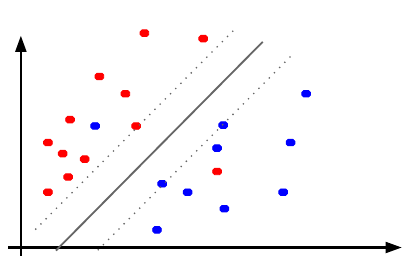
\includegraphics[scale=0.5]{non_separable}

In this case we use \textbf{slack variables} which allow for some margin of error. 
\[
min_{w,b} ||w||^2 + C \sum_{i} {\varsigma}_i
\]\\
subject to: $y_i (w\cdot x_i + b \geq 1- {\varsigma}_i) \forall i$\\

$C$ is a regularization parameter to keep overfitting under control.\\
Slack values can also be calculated: 

\begin{equation}
Slack values:
	\begin{cases}
	0 &  y_i (w\cdot x_i + b) \geq 1 \\
			1- y_i (w\cdot x_i + b) & otherwise
	\end{cases}
\end{equation}

From this we can derive an unconstrained problem: 
\[
min_{w,b} ||w||^2 +C\sum_{i}(max(0,1-y_i (w\cdot x_i + b))
\]

which is similar to a loss function with a regularizer.

An application of SVMs is for example pedestrian detection. 
